\begin{minipage}{.6\linewidth}
	Un ballon-sonde est un ballon à gaz utilisé pour faire des mesures locales dans l'atmosphère.

\bigskip
Dans le cadre du projet scientifique qu'elle anime pour sa classe de CM2, une professeure des écoles a reçu un petit ballon-sonde, représenté ci-dessous.

\bigskip
Son enveloppe, composée de matières plastiques et de latex, a la forme, une fois gonflée, d'un cône de révolution surmonté d'une demi-sphère.

\bigskip
Les dimensions données sur la figure ci-contre sont celles du ballon-sonde au sol, sur le lieu du lâcher situé au niveau de la mer.

\bigskip
La pression atmosphérique diminuant avec l'altitude, le ballon se dilate en prenant de la hauteur et ses dimensions augmentent jusqu'à l'éclatement après une ascension de plus de vingt kilomètres.

\end{minipage}
\begin{minipage}{.4\linewidth}
	\centering
	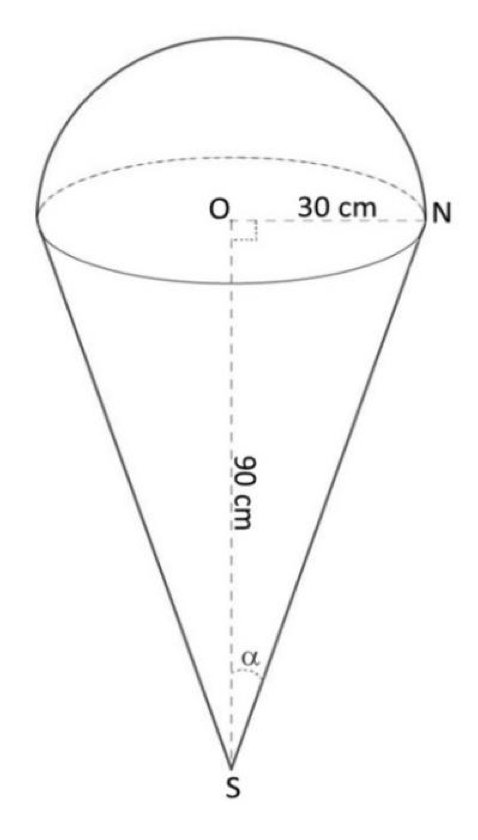
\includegraphics[width=.6\linewidth]{2022-g1-ex5-img1.png}
\end{minipage}

\bigskip
\textit{On pourra, si nécessaire, utiliser le formulaire ci-dessous.}

\begin{center}
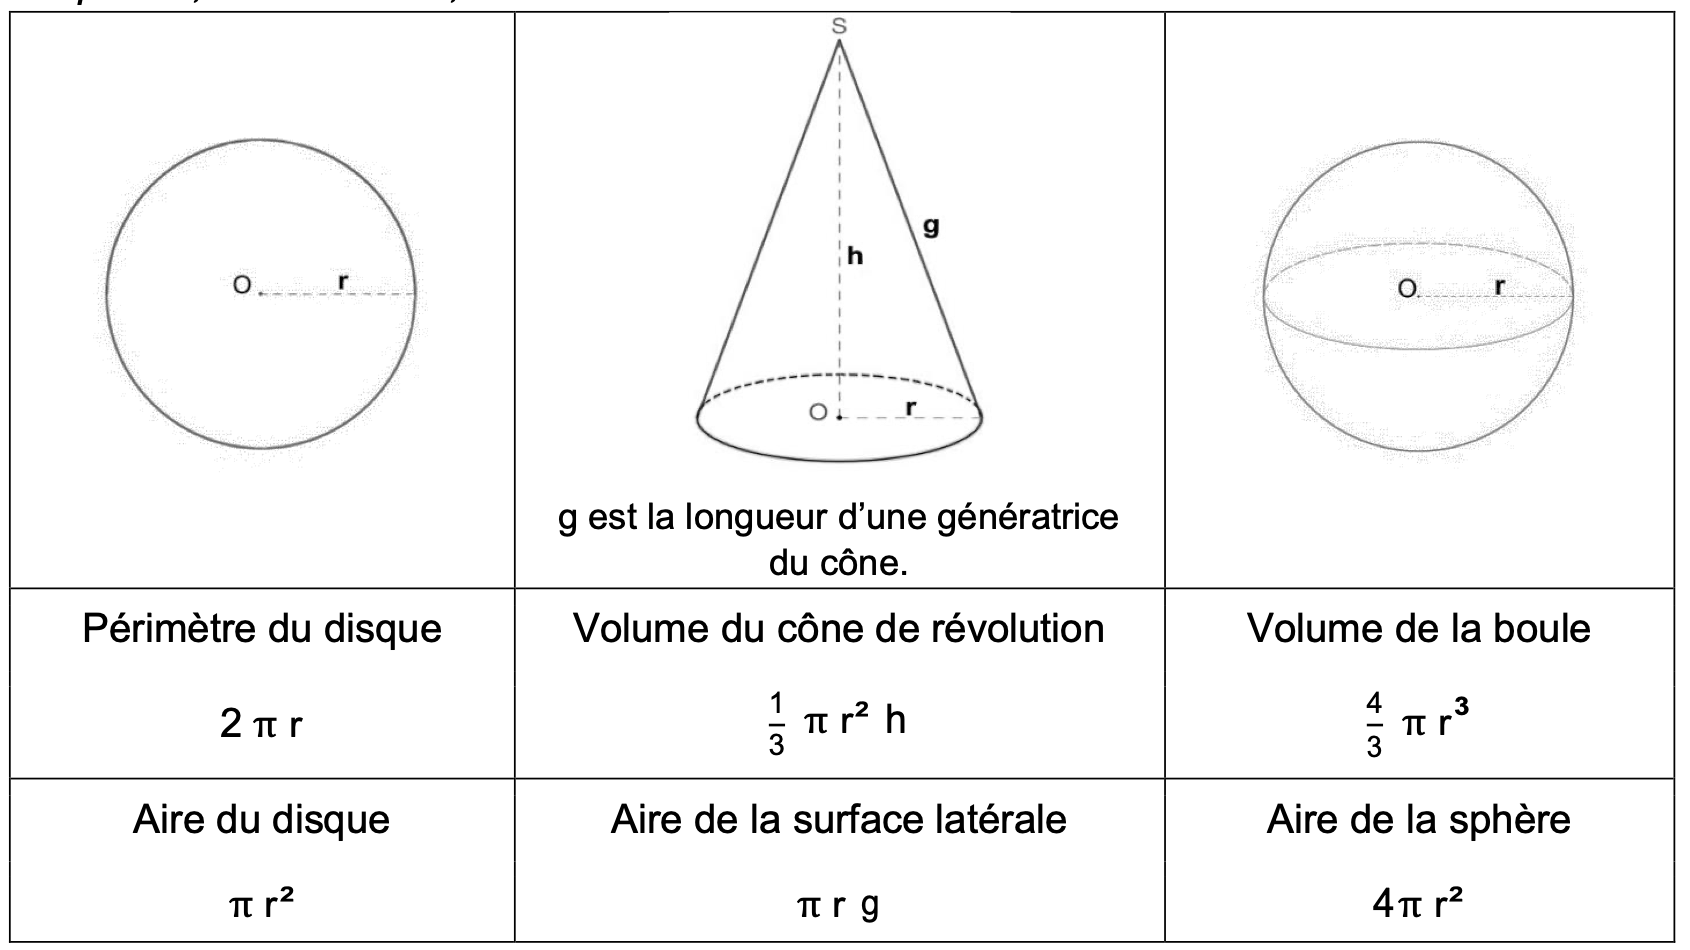
\includegraphics[width=.8\linewidth]{2022-g1-ex5-img2.png}	
\end{center}


\begin{enumerate}
  \item
  
  \begin{enumerate}
  	\item Montrer, en indiquant les étapes du calcul, que le volume exact du ballon-sonde au niveau de la mer, est égal à $45000 \pi~\mathrm{cm}^{3}$.
  	\item Donner le volume du ballon sonde en litre, arrondi à l'entier.
  \end{enumerate}

  \item Montrer qu'une génératrice du cône mesure $\sqrt{9000} \mathrm{~cm}$.

  \item En déduire que l'enveloppe totale du ballon-sonde, au niveau de la mer, a une aire d'environ $1,5 \mathrm{~m}^{2}$ au dixième près. 4. Entre 0 mètre d'altitude et 4500 mètres d'altitude, les longueurs du ballon-sonde augmentent de $25 \%$.
  
  \begin{enumerate}
  	\item Par quel nombre les longueurs initiales sont-elles multipliées ?
  	\item Montrer que, à 4500 mètres d'altitude, l'enveloppe totale du ballon-sonde a une aire d'environ $2,3 \mathrm{~m}^{2}$ arrondie au dixième près.
  	\item Donner un arrondi, au litre près, du volume du ballon-sonde à 4500 mètres d'altitude.
  \end{enumerate}

  \item On lâche le ballon à 0 mètre d'altitude. On relève alors une température de $15^{\circ} \mathrm{C}$. À 4500 mètres d'altitude, la température transmise est de $-12^{\circ} \mathrm{C}$. Entre 0 et $12000 \mathrm{~m}$ d'altitude, la température, en degré Celsius, en fonction de l'altitude $x$, en mètre, peut être modélisée par une fonction affine notée t.

Montrer que pour tout $x$ entre 0 et 12000, on a $t(x)=-0,006 x+15$.

  \item À partir de quelle altitude la température devient-elle négative ? Justifier le résultat en résolvant une inéquation.

  \item La professeure des écoles a réalisé, à l'aide d'un tableur, le calcul des températures en fonction de l'altitude du ballon-sonde.

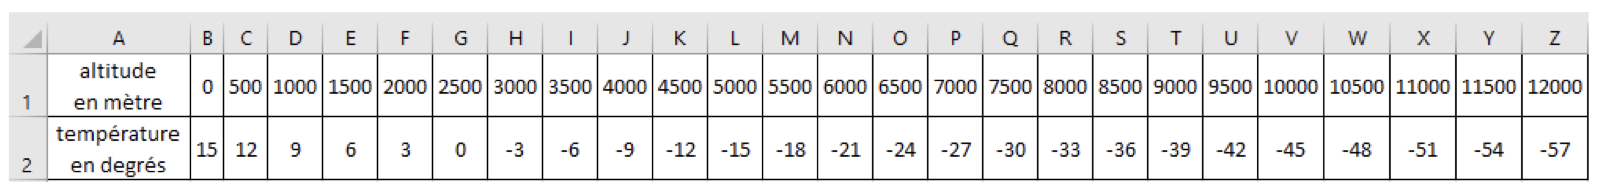
\includegraphics[width=\linewidth]{2022-g1-ex5-img3.png}


En observant les données du tableau, sachant que le ballon part de 0 mètre d'altitude, à quelle altitude se trouve-t-il lorsque la température a baissé de $30^{\circ} \mathrm{C}$ ?

\end{enumerate}

